\documentclass[tikz]{standalone}
% \usepackage{tikz} % already loaded by the documentclass


\begin{document}
%%| filename: ann-diagram
%%| caption: ANN Diagram
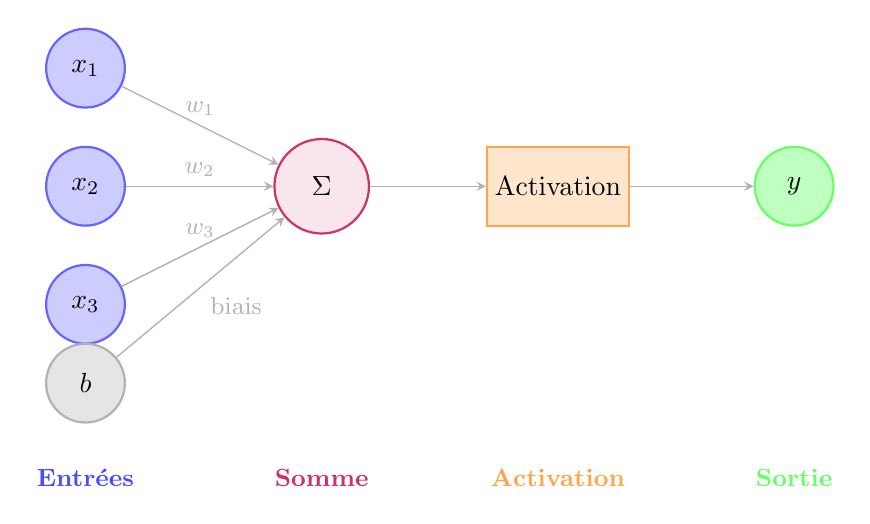
\begin{tikzpicture}[
    input neuron/.style={
        circle,
        draw=blue!60,
        fill=blue!20,
        thick,
        minimum size=1cm,
        inner sep=0pt
    },
    bias neuron/.style={
        circle,
        draw=gray!60,
        fill=gray!20,
        thick,
        minimum size=1cm,
        inner sep=0pt
    },
    sum neuron/.style={
        circle,
        draw=purple!80,
        fill=purple!10,
        thick,
        minimum size=1.2cm,
        inner sep=0pt
    },
    activation neuron/.style={
        rectangle,
        draw=orange!70,
        fill=orange!20,
        thick,
        minimum width=1.8cm,
        minimum height=1cm,
        inner sep=0pt
    },
    output neuron/.style={
        circle,
        draw=green!60,
        fill=green!25,
        thick,
        minimum size=1cm,
        inner sep=0pt
    },
    connection/.style={
        ->,
        >=stealth,
        gray!60,
        line width=0.5pt
    },
    weight/.style={
        connection,
        font=\small,
        auto,
        swap
    }
]

\def\layersep{3}
\def\nodesep{1.5}

%% --- Entrées ---
\node[input neuron] (X1) at (0, 2*\nodesep) {$x_1$};
\node[input neuron] (X2) at (0, 1*\nodesep) {$x_2$};
\node[input neuron] (X3) at (0, 0)         {$x_3$};

%% --- Biais ---
\node[bias neuron] (B) at (0, -1) {$b$};

%% --- Somme ---
\node[sum neuron] (S) at (\layersep, 1*\nodesep) {$\Sigma$};  % Contenu explicite

%% --- Activation ---
\node[activation neuron] (A) at (2*\layersep, 1*\nodesep) {Activation};

%% --- Sortie ---
\node[output neuron] (Y) at (3*\layersep, 1*\nodesep) {$y$};

%% --- Connexions entrées -> somme ---
\draw[connection] (X1) -- node[weight, above] {$w_1$} (S);
\draw[connection] (X2) -- node[weight, above] {$w_2$} (S);
\draw[connection] (X3) -- node[weight, above] {$w_3$} (S);
\draw[connection] (B)  -- node[weight, below right] {biais} (S);

%% --- Somme -> activation ---
\draw[connection] (S) -- (A);

%% --- Activation -> sortie ---
\draw[connection] (A) -- (Y);

%% --- Étiquettes de couches ---
\node[font=\small\bfseries, text=blue!70]      at (0,        -2.2) {Entrées};
\node[font=\small\bfseries, text=purple!80]    at (\layersep,  -2.2) {Somme};
\node[font=\small\bfseries, text=orange!70]    at (2*\layersep,-2.2) {Activation};
\node[font=\small\bfseries, text=green!60]     at (3*\layersep,-2.2) {Sortie};

\end{tikzpicture}
\end{document}
      